% Methods: Explain/justify your methods
    % What values did you end up picking as hyperparameters? Explain how you decided on those values
    % What dimension reduction method(s) did you end up using or not using? Explain how these methods work

\subsection{Data Prepossessing}

\hfill

First we split up the income level by median in the sample data set (around 50000)

Then use the second option to split the population to three by maternal status:

In long-time relationship \[Married, Together\]
Not in long-time relationship \[YOLO, Alone, Single\]
Lost partner from long-time relationship \[Divorced, Widow, Absurd\]

We want to try to classify these population's income level based on other data provided.

The data structure of processed data are as follow:

Categorical data are:

\begin{itemize}
    \item
          $Education$: Customer's education level
    \item
          $Marital\_Status$: Customer's marital status
\end{itemize}

Numerical data are:
\begin{itemize}
    \item $Year\_Birth$: Customer's birth year
    \item $Income$: Customer's yearly household income
    \item $Kidhome$: Number of children in customer's household
    \item $Teenhome$: Number of teenagers in customer's household
    \item $Recency$: Number of days since customer's last purchase
    \item $MntWines$: Amount spent on wine in last 2 years
    \item $MntFruits$: Amount spent on fruits in last 2 years
    \item $MntMeatProducts$: Amount spent on meat in last 2 years
    \item $MntFishProducts$: Amount spent on fish in last 2 years
    \item $MntSweetProducts$: Amount spent on sweets in last 2 years
    \item $MntGoldProds$: Amount spent on gold in last 2 years
    \item $NumDealsPurchases$: Number of purchases made with a discount
    \item $NumWebPurchases$: Number of purchases made through the company's website
    \item $NumCatalogPurchases$: Number of purchases made using a catalogue
    \item $NumStorePurchases$: Number of purchases made directly in stores
    \item $NumWebVisitsMonth$: Number of visits to company’s website in the last month
    \item $Complain$: 1 if the customer complained in the last 2 years, 0 otherwise
\end{itemize}

Among those data, normally distributed are:$Year\_Birth$, $Recency$

\begin{figure}[h]
    \centering
    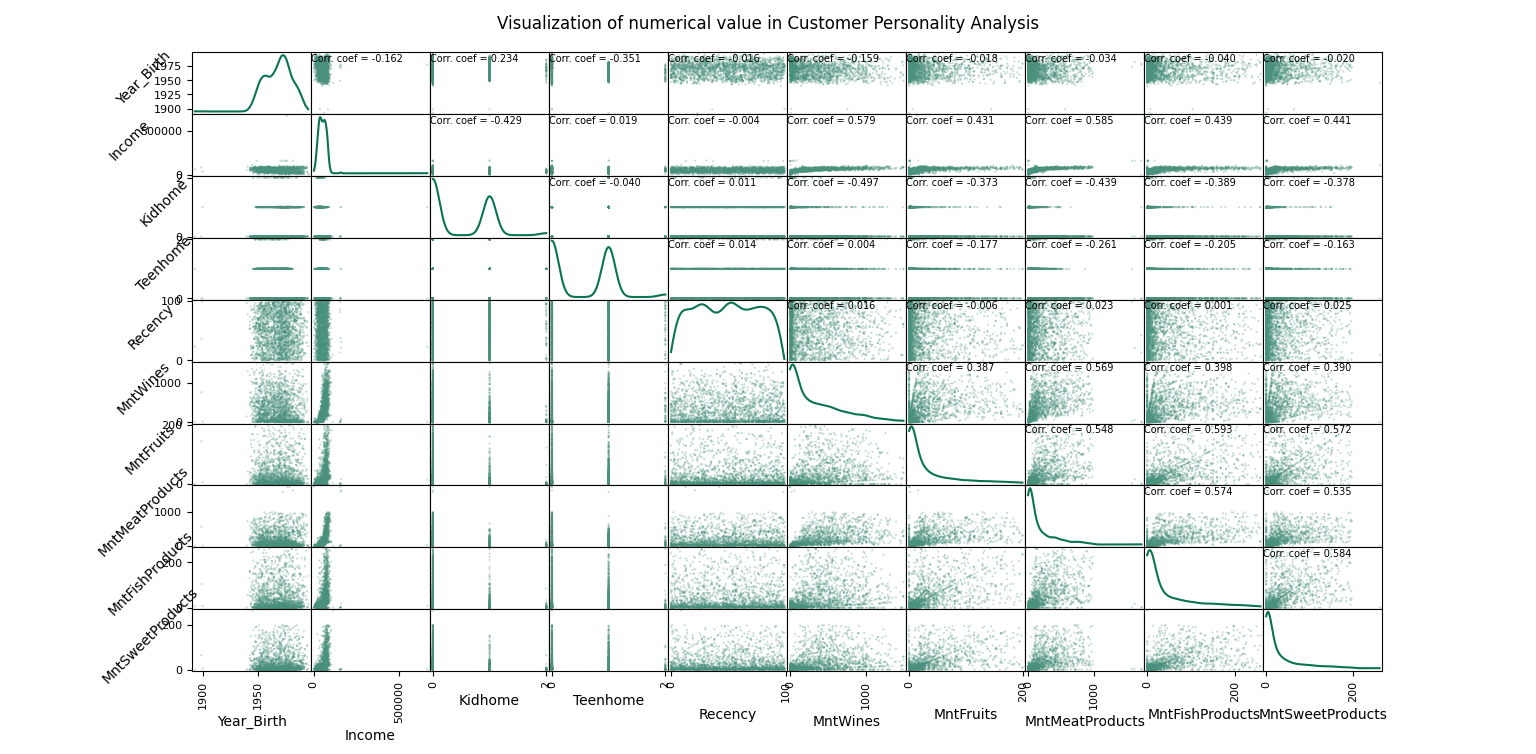
\includegraphics[width=\textwidth]{images/numerical_visualization.png}
    \caption{An ugly figure to show multidimensional distribution of the dataset}
    \label{feature_fit}
\end{figure}

\subsection{Model Selection}

Wen each of the model, we tune the following parameters:
\begin{enumerate}
    \item
          k-nearest neighbors is a model that predicts class of a given value based on the data points around it.

          k-nearest neighbors is better than naive-bayes classifier because
          - it can be used to fit non linear relationships.
          - it is easy to implement and interpret.

          However k-nearest neighbors has following weakness comparing to naive-bayes classifier because
          - it need to run with the data set, which required more storage than naive-bayes classifier
          - it generally has longer training time.

    \item
          Random Forest is a model that fits a number of decision tree classifiers on various sub-samples of the dataset and uses averaging to improve the predictive accuracy and control over-fitting.

          Random forest is better than decision-tree because
          - it uses ensemble learning by averaging to improve the predictive accuracy and control over-fitting.
          - each of the tree is easy to explain.

          Nevertheless, Random forest has following weakness comparing to  decision-tree because
          - generally has longer training time.
          - generally requires more storage required comparing to decision

    \item Artificial Neural Networks (ANN) are computational models inspired by the human brain, consisting of layers of interconnected nodes that process input data through activation functions to make predictions or classifications. They are capable of learning complex patterns from data through a process called training, where the model adjusts its internal parameters to minimize error.


          Artificial Neural Networks (ANN) are often preferred over simpler models like logistic regression because:

          they can model highly complex and non-linear relationships within the data.
          they excel in tasks with large and diverse datasets, adapting through deep learning to achieve better performance.


          Artificial Neural Networks (ANN) have the following weaknesses compared to simpler models like logistic regression:

          They require significant computational resources for training, which can be time-consuming and costly, especially for large networks.
          They are prone to overfitting, particularly in cases where the amount of data is limited relative to the complexity of the model.



    \item Support Vector Machines (SVM) are supervised learning models that analyze data for classification and regression tasks. They work by finding the hyperplane that best divides a dataset into classes with the largest margin, thus providing a robust prediction model especially effective in high-dimensional spaces.


          Support Vector Machines (SVM) are favored over k-nearest neighbors in some cases because:

          they are effective in high-dimensional spaces, where the distance between data points is crucial for classification.
          they offer a clear margin of separation, which helps to reduce the risk of overfitting in contrast to more local or memory-intensive methods.


          Support Vector Machines (SVM) also exhibit certain disadvantages compared to models like logistic regression:

          They are not very efficient with large datasets as the training time can scale poorly, making them less suitable for larger-scale applications.
          They can be sensitive to the choice of kernel and regularization parameters, which can make tuning the model complex and require careful selection to achieve optimal performance.

\end{enumerate}

\subsection{Hyperparameter Tuning}

\hfill

The process of hyperparameter tuning is central to optimizing the performance of machine learning models. Hyperparameters are the adjustable parameters that control the model training process, as opposed to the internal parameters determined by the training data itself. Proper selection and adjustment of these parameters can significantly enhance model performance, especially in complex datasets.

\begin{enumerate}
    \item For the hyper-parameter tuning, KNN:

          We will use different neighbor counts for KNN. We'll test values

          $n\_neighbors=3,5,9,17,21,33$

    \item Random Forest:

          We will use the number of trees. We'll test values

          $n\_estimators=1,2,4,8,16,32,64,128,256,512$

          We will test $max\_samples$ passed to each tree, the number of samples to draw from X to train each base estimator. We'll try the fractions

          $max\_samples=0.1,0.3,0.5,0.7,0.9$

    \item
          For the Artificial Neural Network (ANN), you can explore the following hyperparameter settings during your experimentation:

          Units: Number of neurons in each layer. We tested different layer sizes with values units=$[5, 10]$.
          Activation: Type of activation function used in the neurons. I'll try both $activation=[relu, tanh]$.

          Learning Rate: The step size at each iteration while moving toward a minimum of a loss function. Possible values to test are $learning\_rate=[0.1, 0.01]$.

          Epochs: Number of times the learning algorithm will work through the entire training dataset. For this test, I'll use epochs=$[20]$.

          Batch Size: Number of samples propagated through the network before the update of internal model parameters. I'll experiment with $batch\_size=[16]$.

    \item For the Support Vector Machine (SVM), the hyperparameter grid you could explore includes:

          C (Regularization parameter): The strength of the regularization is inversely proportional to C. Must be strictly positive. The penalty is a squared l2 penalty. I'll test values $C=[0.1, 1, 10, 100]$.
          Kernel: Specifies the kernel type to be used in the SVM algorithm. Options to test include $kernel=[linear, poly, rbf, sigmoid]$.
\end{enumerate}

